\documentclass[12pt, oneside]{article} 
\usepackage[left=15mm, right=15mm, top=10mm]{geometry}
\usepackage{graphicx}
\usepackage{url}
\usepackage{multicol}
\usepackage{hyperref}
\usepackage{float}

\begin{document}
\title{Techniques d'attaque - exploitation avec Metasploit}
\author{Tristan BILOT, Nora DELFAU, Enzar SALEMI, Madushan THAMBITHURAI\\EPITA}
\date{10 Juin 2021}
\maketitle

\begin{abstract}
L'objectif de ce TP est d'utiliser les outils metasploit et armitage afin de prendre le contrôle à distance d'une machine Windows XP et 2000 vulnérables. Dans un premier, l'objectif sera d'avoir un reverse shell avec des droits utilisateur puis d'essayer une élévation de privilèges afin d'obtenir des droits administrateur. 
\end{abstract}

\section{Notes}
\subsection{Ping entre machine victime}
Avant de mettre en oeuvre l'exploitation, il faut allumer la machine de l'attaquant et celle de la victime. L'attaquant utilisera Kali Linux et la victime windows XP pour cet exemple.
L'option -e permet d'encoder le binaire malveillant afin qu'il soit moins détectable par les antivirus ou les personnes voulant l'analyser. Cependant, un binaire trop encodé peut ne pas être exécuté sur la machine cible.
\begin{figure}[H]
\centering
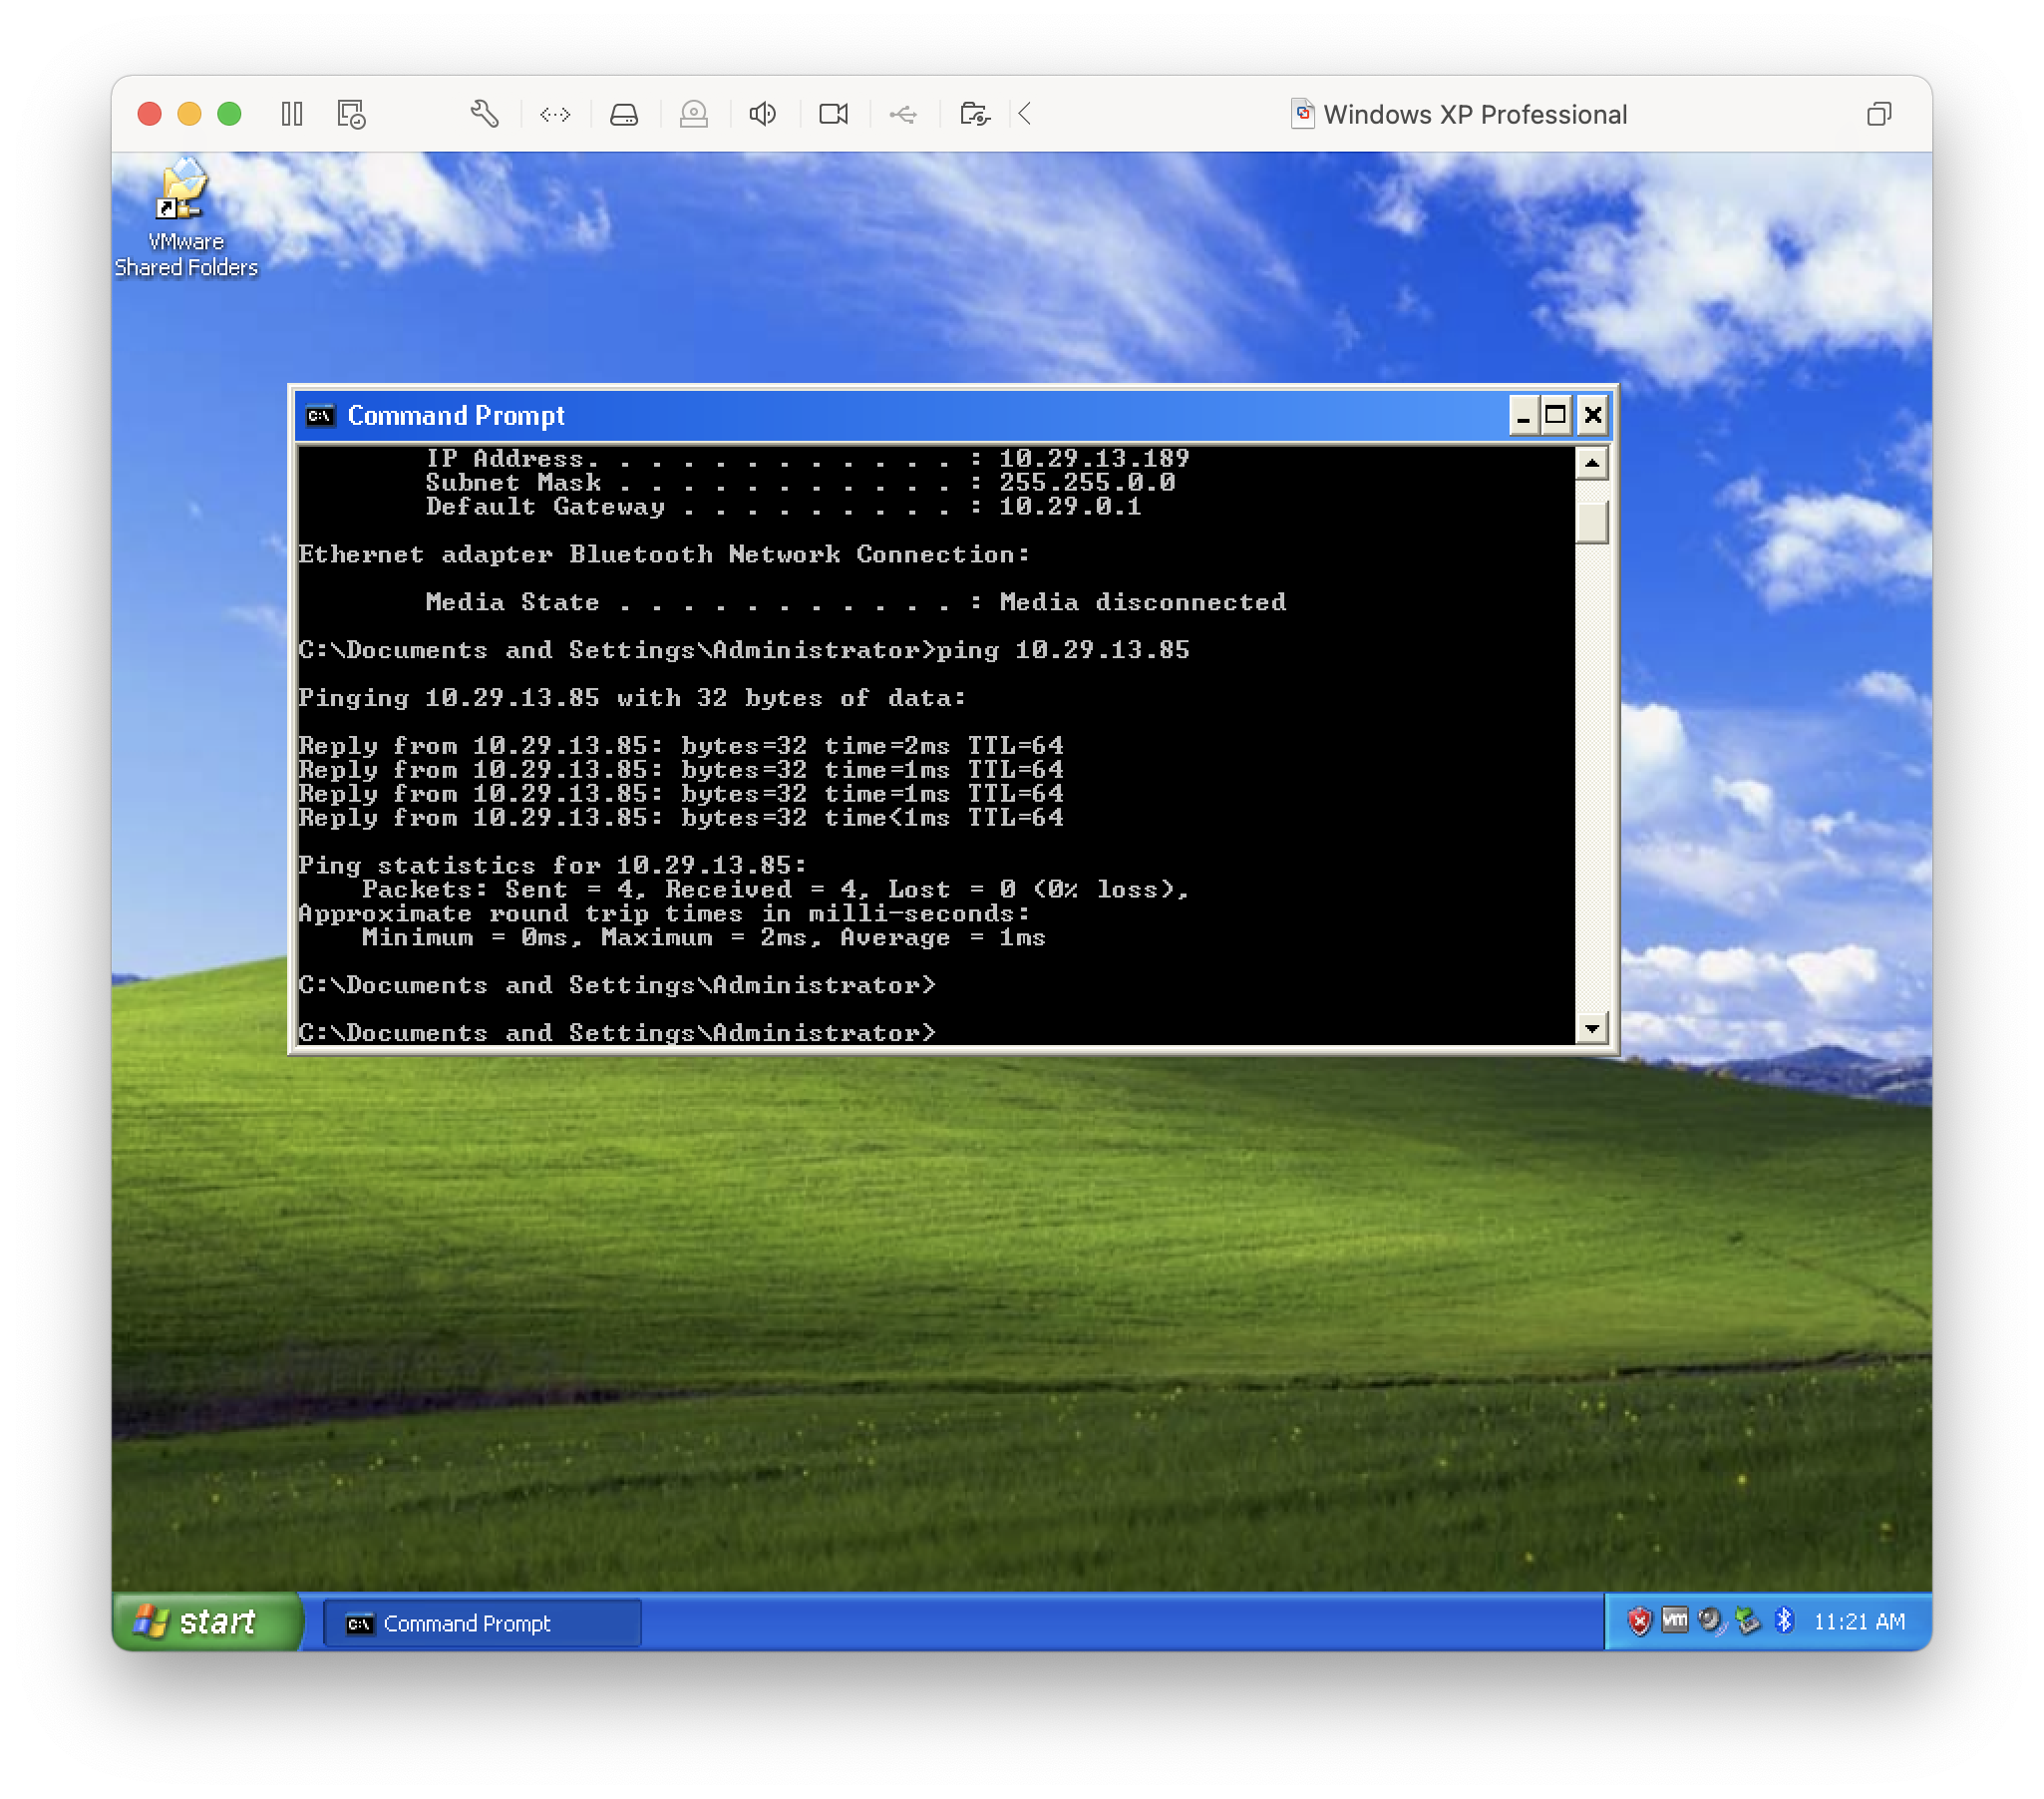
\includegraphics[scale=0.4]{win}
\caption{Ping de l'attaquant (Kali) à partir de la victime (Windows XP)}
\end{figure}
\subsection{Exploitation}
Nous savons que la machine Windows ciblée est vulnérable à la vulnérabilité MS10\_046, lançons donc un exploit afin de récupérer un shell sur la machine distante. La vulnérabilité MS10\_046 concerne l'utilisation des liens au sein de Windows. Au moment du clic sur un lien, il est possible de générer une dll permettant une RCE et ainsi le spawn d'un shell. Cette vulnérabilité n'est présente que sur de très vieilles versions de Windows. Toutefois, certaines entreprises peuvent encore utiliser des versions vulnérables.
\begin{figure}[H]
\centering
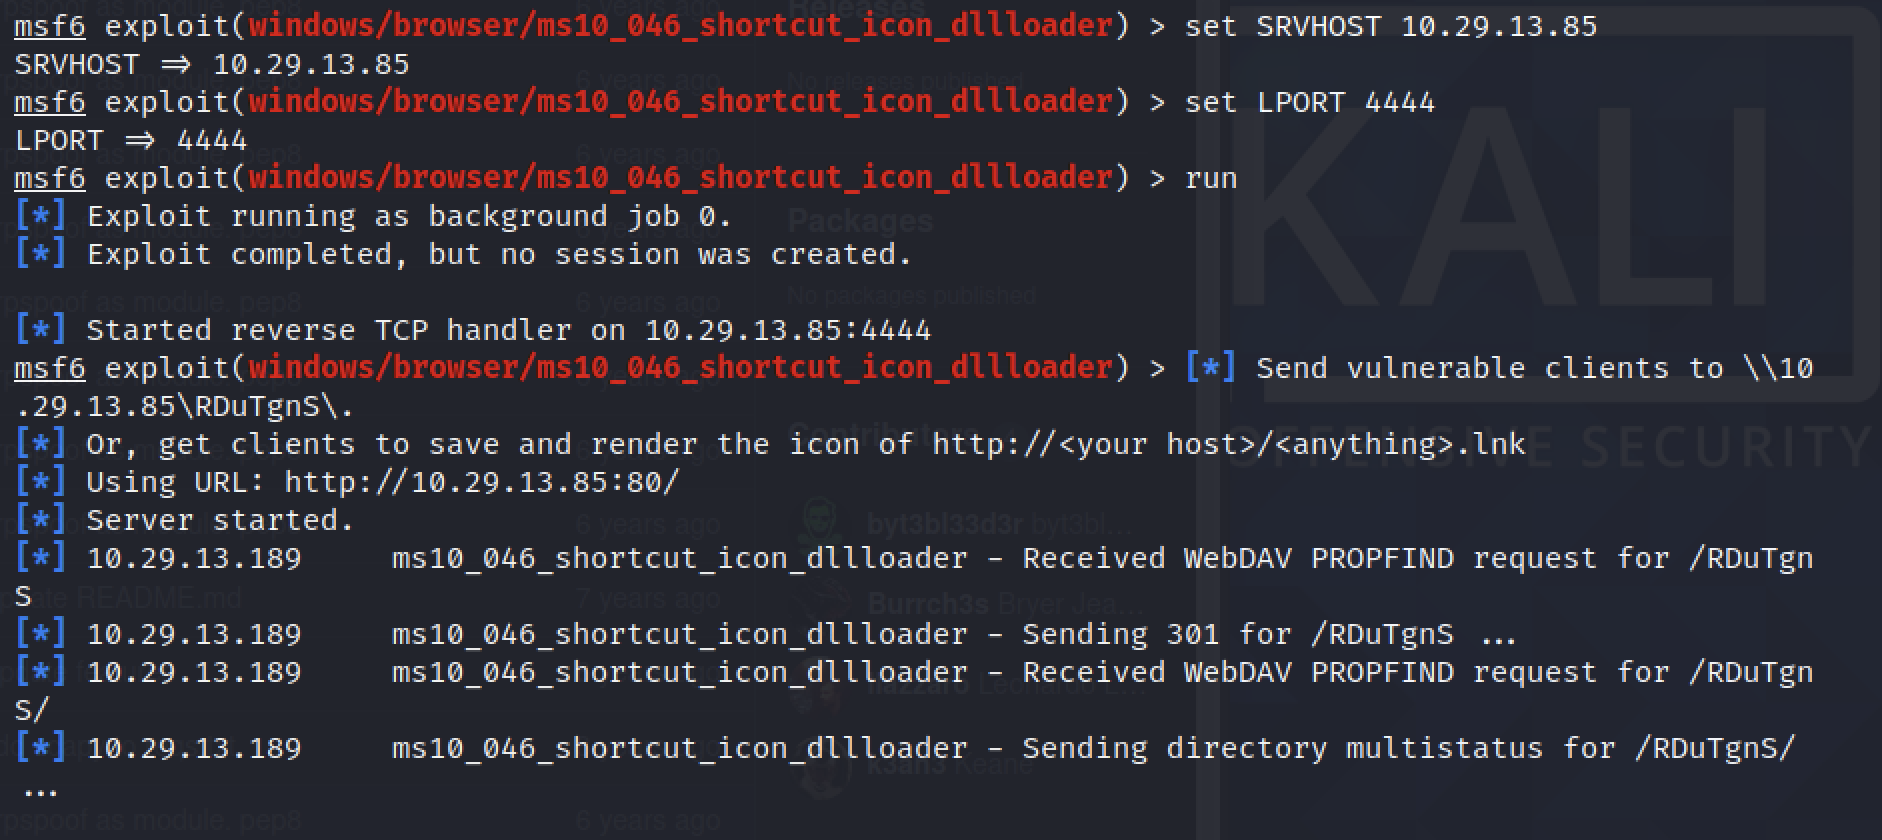
\includegraphics[scale=0.4]{msf}
\caption{Lancement de l'exploit MS10\_046 et obtention d'un shell}
\end{figure}
\begin{figure}[H]
\centering
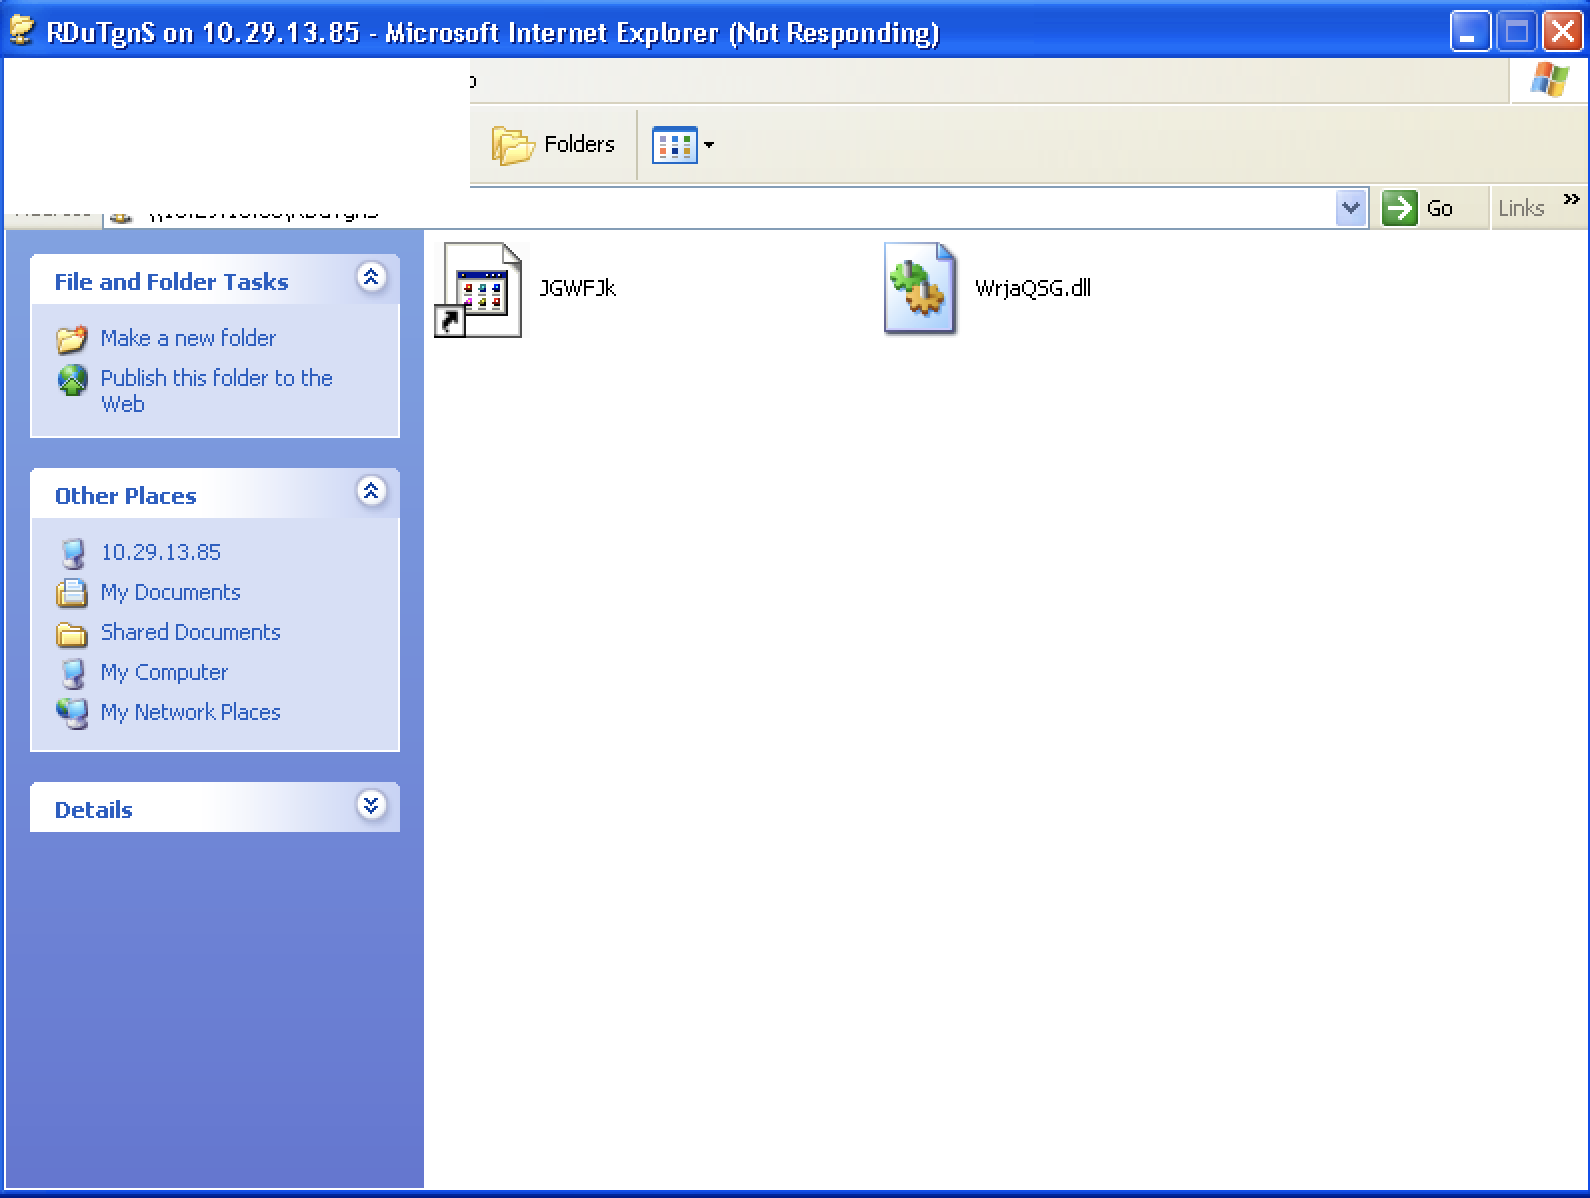
\includegraphics[scale=0.4]{win2}
\caption{Ouverture du lien sur la machine cible}
\end{figure}
\subsection{Élévation de privilèges}
Metasploit propose une commande getsystem permettant de tester en arrière plan différentes vulnérabilités afin de mettre en place une élévation de privilèges. Cette commande fonctionne rarement mais est un succès ici étant donné que la version de l'OS est très ancienne et non mise à jour.
\begin{figure}[H]
\centering
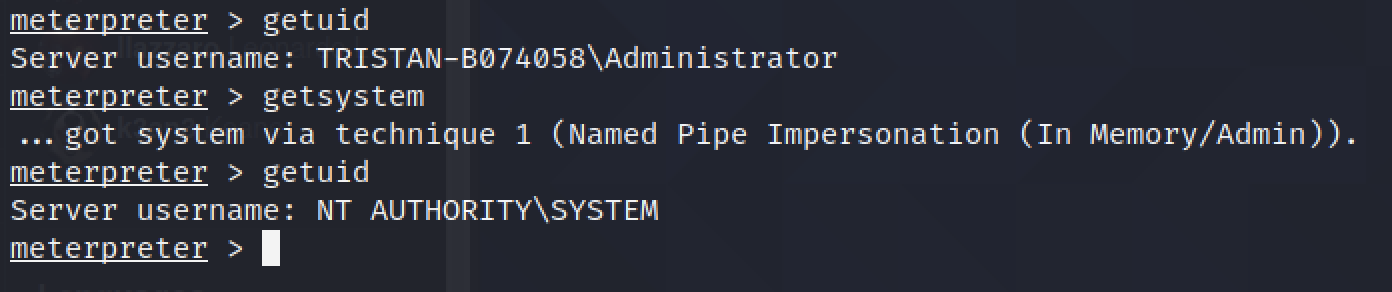
\includegraphics[scale=0.4]{system}
\caption{Élévation de privilèges}
\end{figure}
\section{Trojan}
\subsection{Création du trojan}
Metasploit propose une commande permettant de générer des fichiers malveillants de toute sort, permettant notamment des accès distants à une machine. Cette commande est msfvenom. Il faut spécifier le payload à exécuter: ici un reverse shell afin que la machine distante se connecte à notre machine pour obtenir un meterpreter, l'adresse IP de l'attaquant nécessaire pour la connexion, le port, ainsi que le type de fichier généré, ici un exécutable pour Windows.
\begin{figure}[H]
\centering
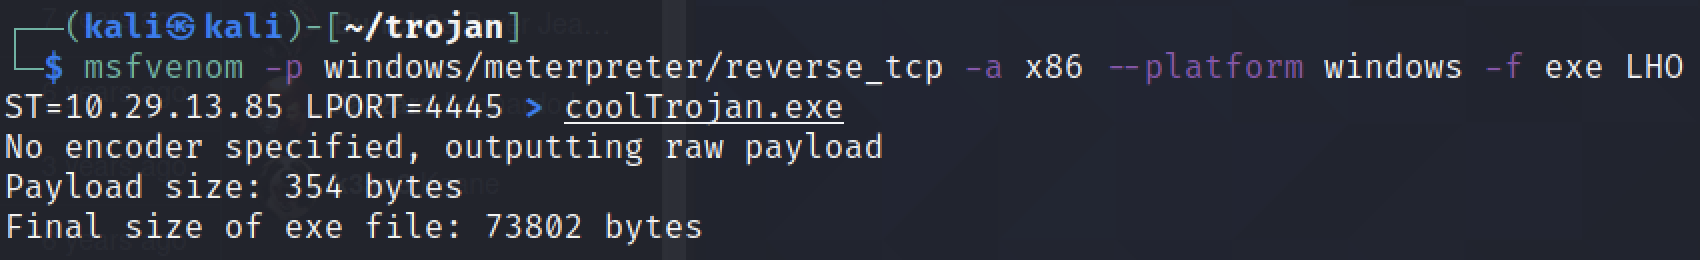
\includegraphics[scale=0.4]{trojan}
\caption{Génération d'un trojan via msfvenom}
\end{figure}
\subsection{Lancement du handler}
Maintenant que notre malware est créé, il faut lancer un serveur en écoute sur le port indiqué dans l'exécutable afin de handle la connexion et de pouvoir communiquer avec la victime. Pour cela, on utilise généralement le module multi/handler de metasploit.
\begin{figure}[H]
\centering
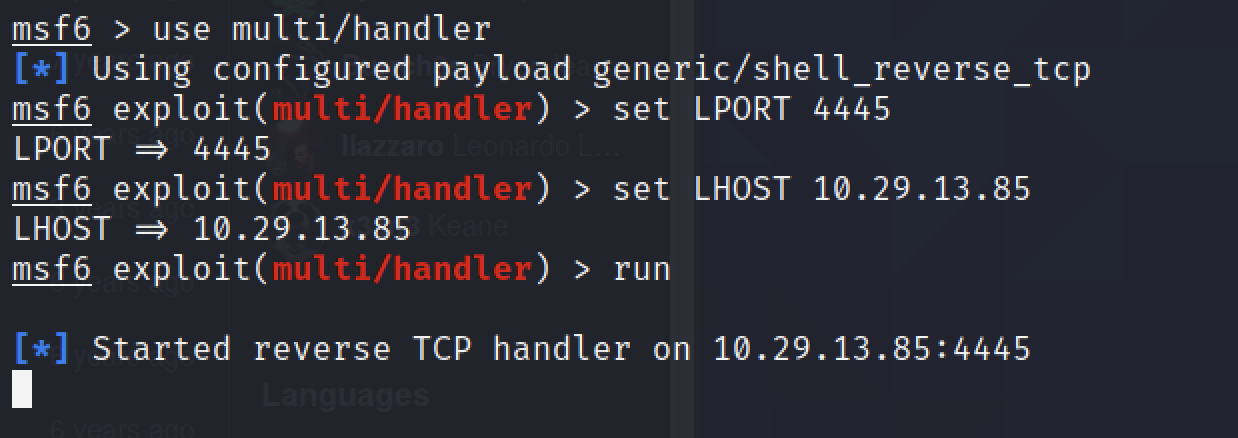
\includegraphics[scale=0.4]{handler}
\caption{Lancement du multi/handler}
\end{figure}
Il ne reste plus qu'à réussir à faire cliquer la victime sur l'exécutable. Cela peut être effectué via des techniques de social engineering. Lorsque la victime l'ouvre, le payload est lancé et le reverse shell apparaît côté attaquant.
\begin{figure}[H]
\centering
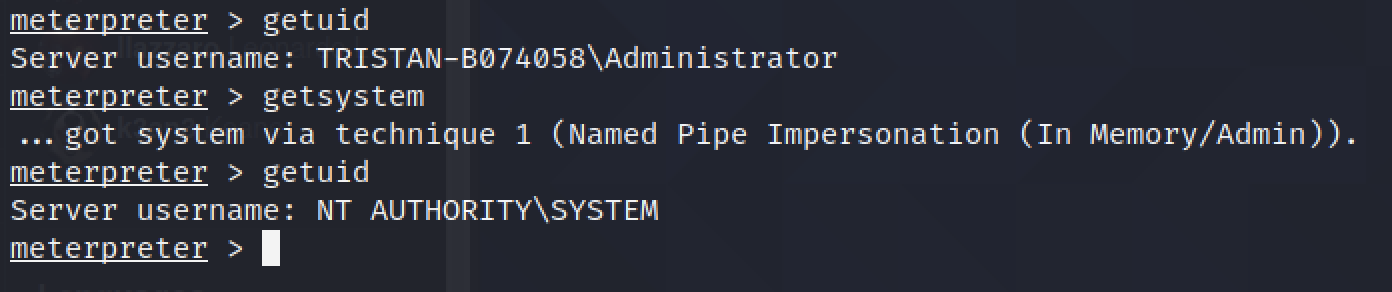
\includegraphics[scale=0.4]{system}
\caption{Obtention d'un meterpreter + élévation de privilèges}
\end{figure}
\section{Rainbow table cracking}
\subsection{Définition}
Lors de l'authentification des utilisateurs, les mots de passe sont stockés sous forme de texte brut ou de hachage. Étant donné que les mots de passe stockés en clair sont facilement volés si l'accès à la base de données est compromis, les bases de données stockent généralement des hachages à la place. Ainsi, personne, y compris le système d'authentification – ne peut apprendre un mot de passe simplement en regardant la valeur stockée dans la base de données. \\\\Lorsqu'un utilisateur entre un mot de passe pour l'authentification, un hachage est calculé pour lui, puis comparé au hachage stocké pour cet utilisateur. L'authentification réussit si les deux hachages correspondent. (D'un autre côté, essayer d'utiliser une valeur hachée comme mot de passe pour se connecter échouerait car le système d'authentification la hacherait une deuxième fois.) \\\\Apprendre un mot de passe à partir d'un hachage, c'est trouver une chaîne qui, lorsqu'elle est entrée dans la fonction de hachage, crée ce même hachage. C'est la même chose que l'inversion de la fonction de hachage.\\\\Bien que les attaques par force brute (par exemple, les attaques par dictionnaire) puissent être utilisées pour essayer d'inverser une fonction de hachage, elles peuvent devenir infaisables lorsque l'ensemble des mots de passe possibles est suffisamment grand. Une alternative à la force brute consiste à utiliser des tables de chaînes de hachage précalculées. Les tables arc-en-ciel sont un type particulier de telles tables qui surmontent certaines difficultés techniques.
\subsection{Création}
L'outil rtgen permet de générer des tables rainbow tables suivant certaines règles.
\begin{figure}[H]
\centering
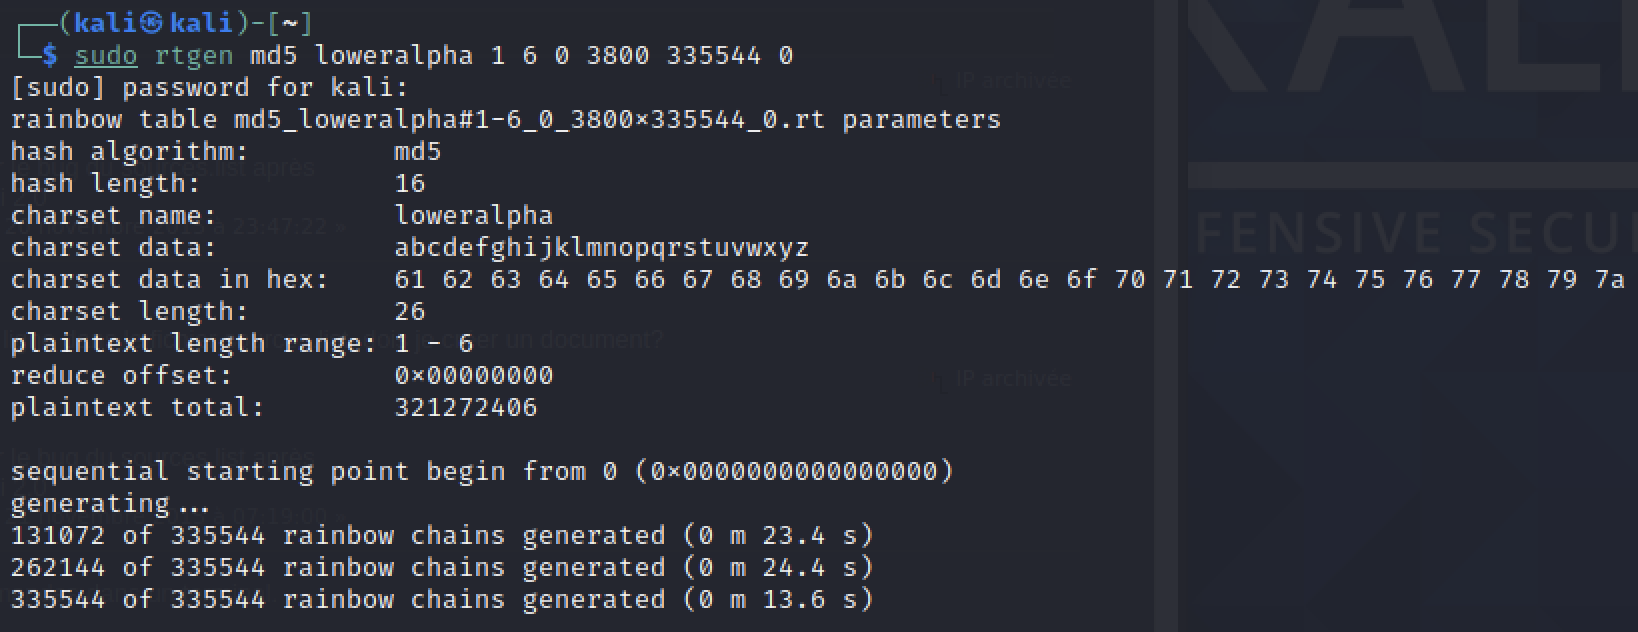
\includegraphics[scale=0.4]{rainbow}
\caption{Génération de la rainbow table via rtgen}
\end{figure}
Une fois cette table créée, il est possible de l'utiliser afin de cracker des mot de passe hashés. Avant cela, utiliser la commande ntsort permet de trier la table afin d'optimiser la vitesse de recherche du mot de passe parmi tous les hashs. C'est ensuite via la commande ntcrack que l'attaque se produit.
\begin{figure}[H]
\centering
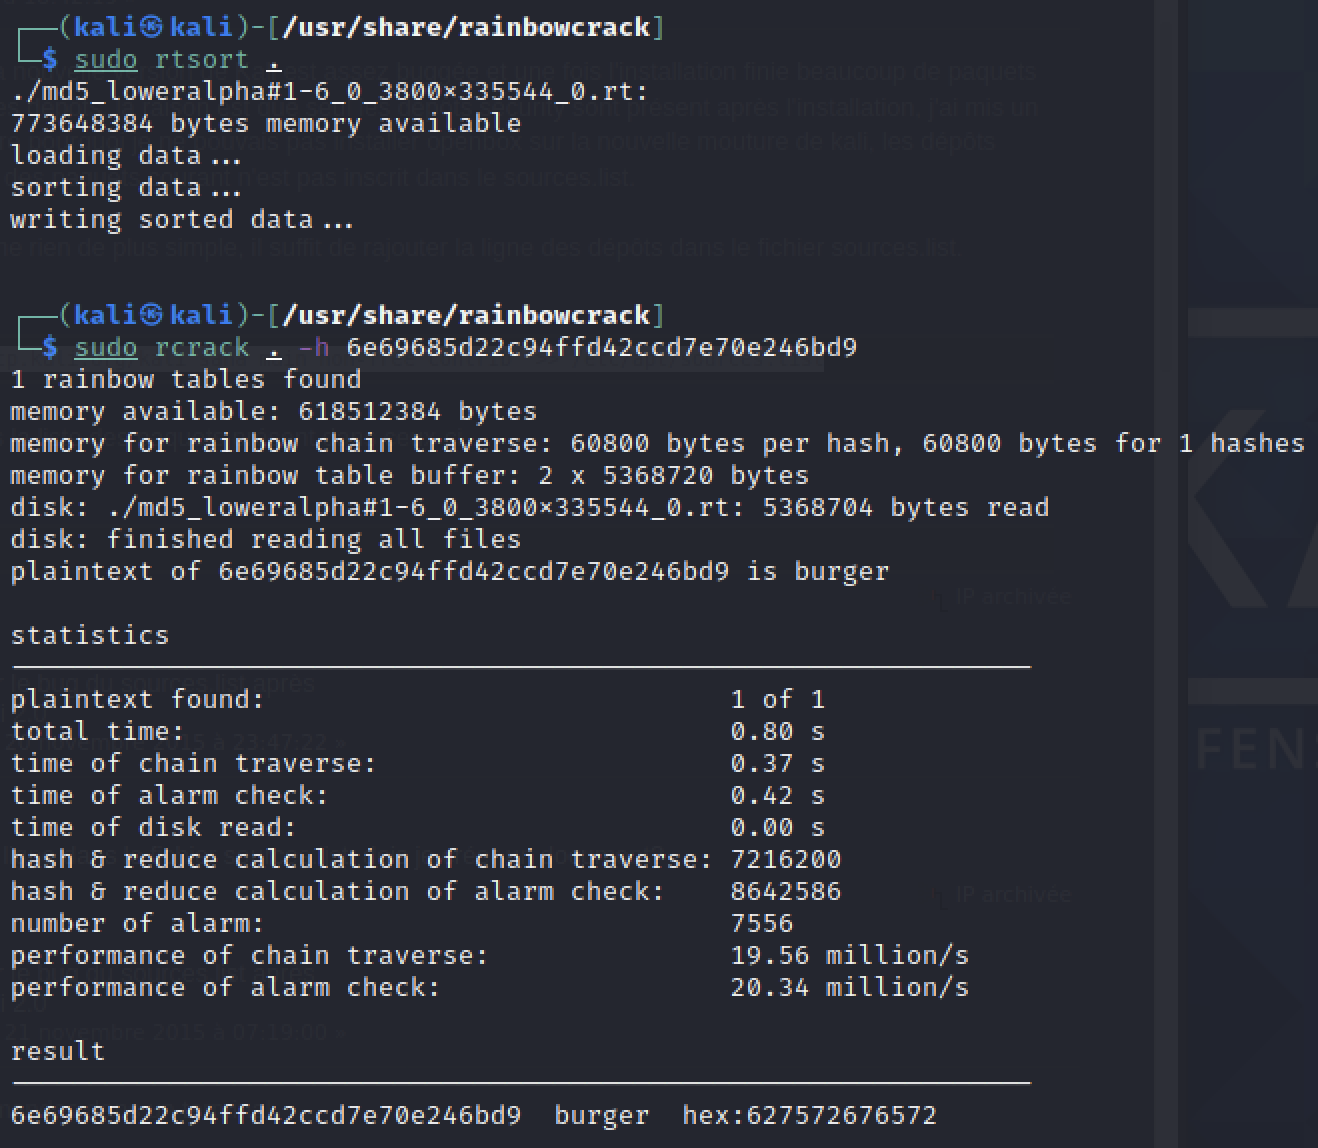
\includegraphics[scale=0.4]{rtcrack}
\caption{Attaque sur le hash via rtcrack}
\end{figure}

\section{Reverse TCP exe sur Windows 2000}
\subsection{Reconnaissance et exploitation}
La commande nmap -O -sV IP scanne une plage d’adresse (ou une adresse individuelle) pour déterminer le système d’exploitation de l’hôte (option -O) et les services disponibles dont la version (option -sV).\\
Ici, la machine cible a pour adresse IP : 10.189.133.166. On utilisera la commande “nmap -O -sV 10.189.133.166”.
\begin{figure}[H]
\centering
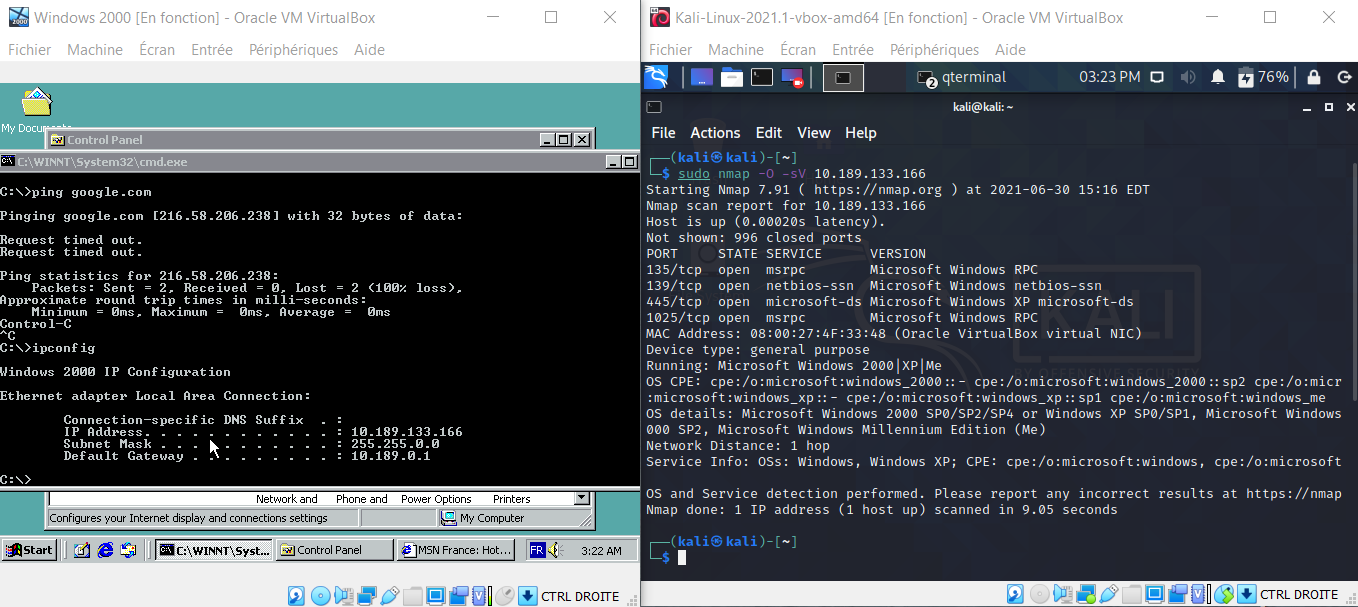
\includegraphics[scale=0.4]{Image1}
\end{figure}

\begin{itemize}
\item Quelles sont les propriétés de cette machine ?
A l’aide de la commande nmap, on apprend que la machine possède 1000 ports dont 996 fermés. Les ports ouverts sont : 135 (msrpc), 139 (netbios-ssn), 445 (microsoft-ds) et 1025 (msrpc). On a également l’adresse MAC de la machine et son OS (Windows 2000). 
Les ports 139 et 445 correspondent au protocole SMB connu pour être vulnérable.
\item Lancer une recherche d’exploits possible ?
En utilisant la commande “search” dans metasploit, on peut obtenir les exploits avec l’argument type:exploit et orienter les résultats sur le protocole smb avec l’argument windows/smb. On obtient la liste suivantes :
\end{itemize}
\begin{figure}[H]
\centering
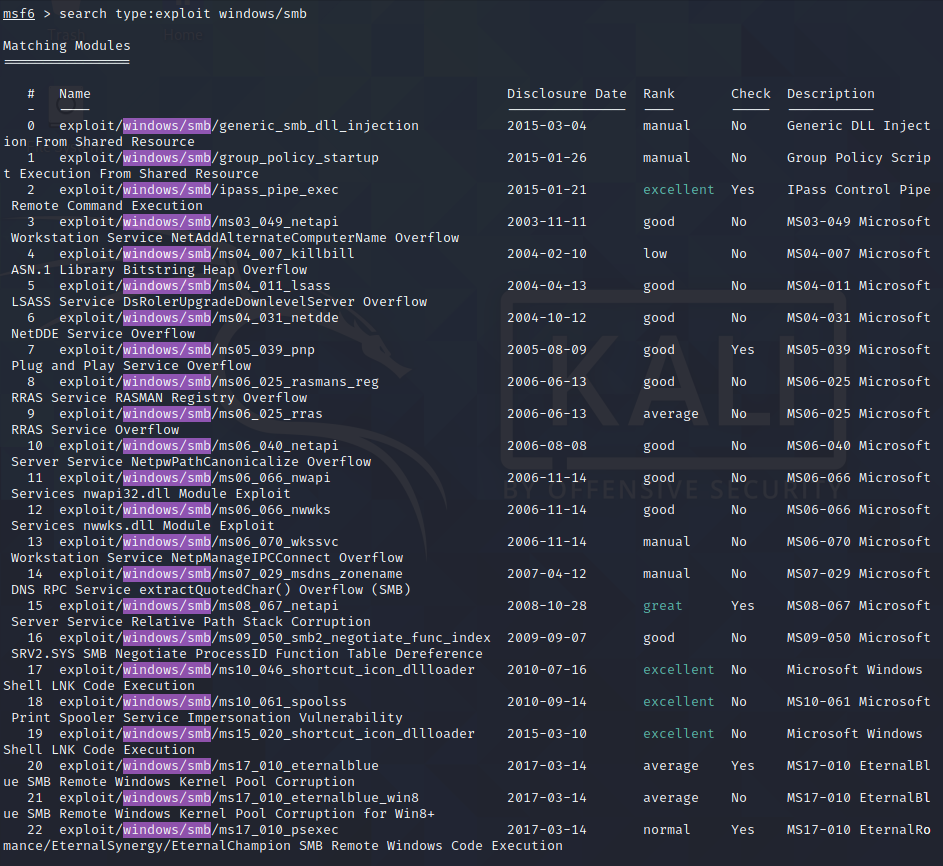
\includegraphics[scale=0.4]{Image2}
\end{figure}
Exploiter ces deux vulnérabilités :\\
Vulnérabilité Plug-and-Play: CVE-2005-1983 (MS-05-039): ça entraîne le plantage (hanging permanent) de la machine distante qui ne répond plus aux commandes de l’utilisateur, ce qui est préjudiciable car c’est un déni de service pour celui-ci
Dans la liste obtenue précédemment, on retrouve le chemin d’un exploit concernant la vulnérabilité PnP (MS-05-039). On utilise la commande “use” pour pouvoir la paramétrer avant de l’exploiter. On renseigne l’OS, soit Microsoft 2000 SP0-SP4, et son adresse IP. Une fois les informations remplies, on peut lancer la commande “exploit”.
\begin{figure}[H]
\centering
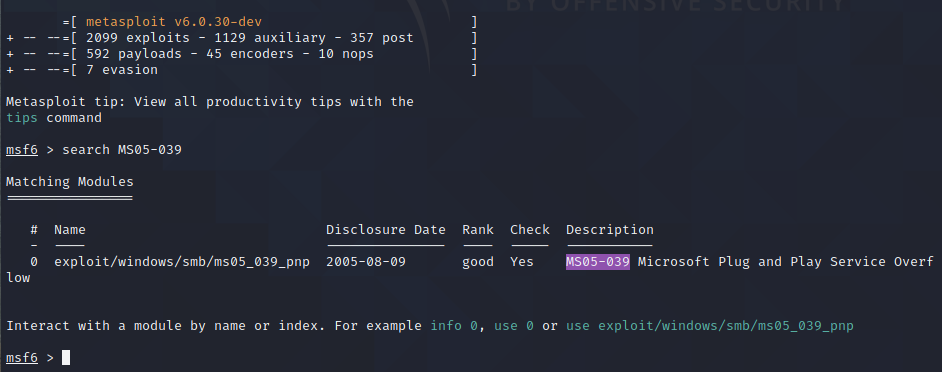
\includegraphics[scale=0.4]{Image3}
\end{figure}
\begin{figure}[H]
\centering
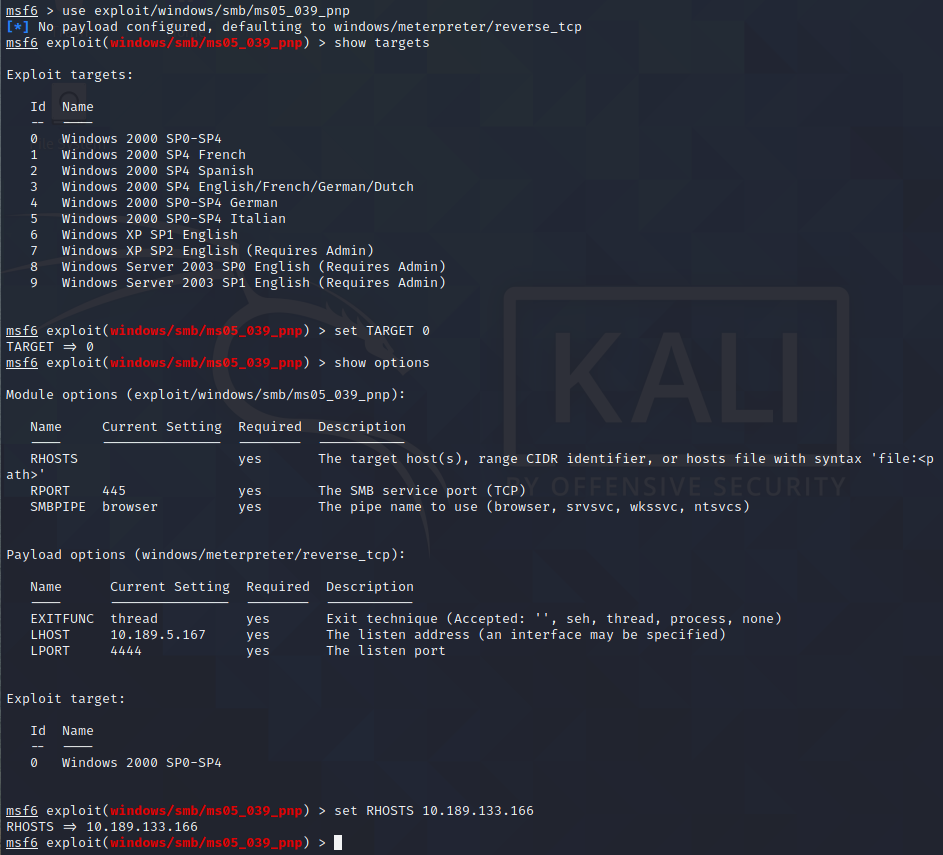
\includegraphics[scale=0.4]{Image4}
\end{figure}
\begin{figure}[H]
\centering
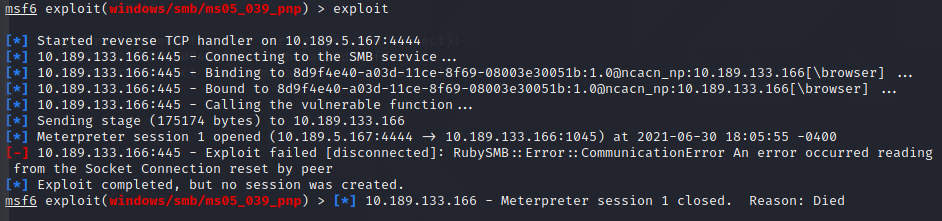
\includegraphics[scale=0.4]{Image5}
\end{figure}
L’exploit n’a pas abouti. Une erreur RubySMB n’a pas pu être résolue malgré des modifications de Target, Payload, SMBPIPE et de port.
Vulnérabilité LSASS: CVE-2003-0533 (MS-04-011) : ça crée un shell distant qui s'interrompt immédiatement. Or, ce qui diffère est que l’échec de l’exploit force l’arrêt du processus lsass.exe (Local Security Authority Subsystem Service) qui est responsable de l’application des politiques de sécurité de Windows (authentification des utilisateurs, écriture dans les journaux de sécurité...). En réponse à cela, le système doit redémarrer pour corriger son état (figure 19). Ceci peut également être considéré comme un déni de service.
Dans la liste obtenue précédemment, on retrouve également le chemin d’un exploit concernant la vulnérabilité LSASS (MS-04-011). On utilise la commande “use” pour pouvoir la paramétrer avant de l’exploiter. On renseigne l’OS, soit Microsoft 2000 English, et son adresse IP. Une fois les informations remplies, on peut lancer la commande “exploit”
\begin{figure}[H]
\centering
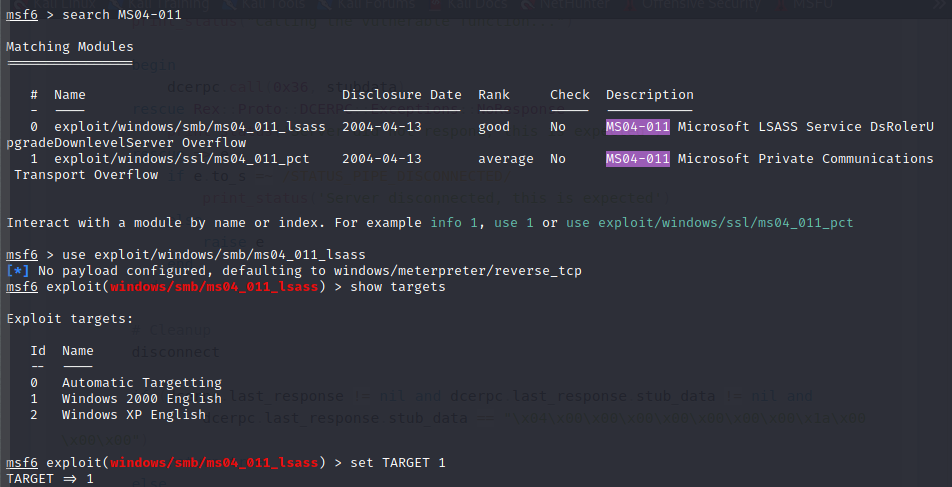
\includegraphics[scale=0.4]{Image6}
\end{figure}
\begin{figure}[H]
\centering
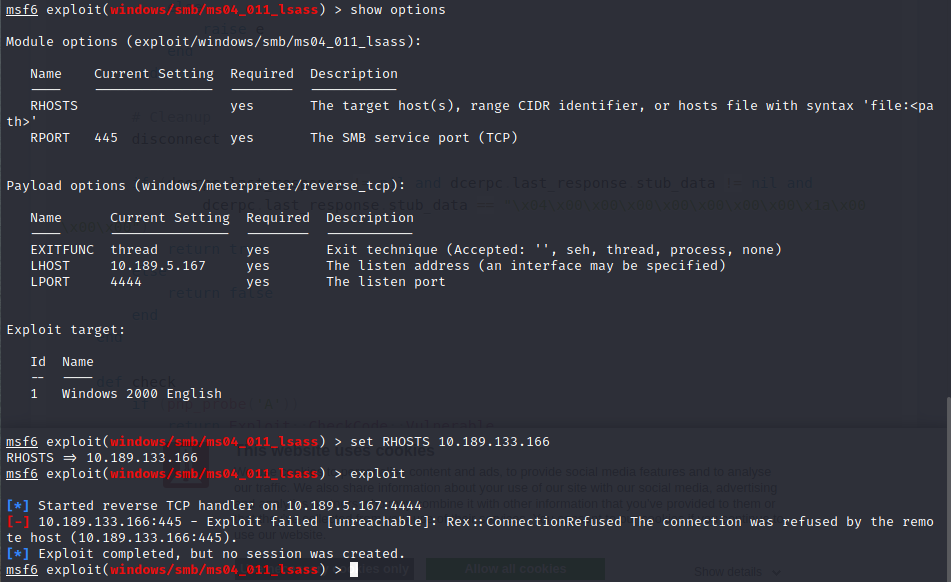
\includegraphics[scale=0.4]{Image7}
\end{figure}
\begin{figure}[H]
\centering
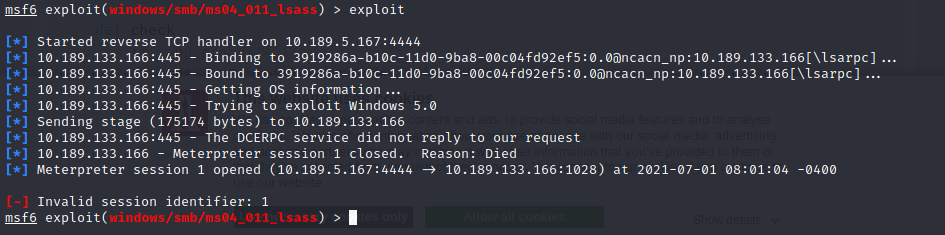
\includegraphics[scale=0.4]{Image8}
\end{figure}
\begin{figure}[H]
\centering
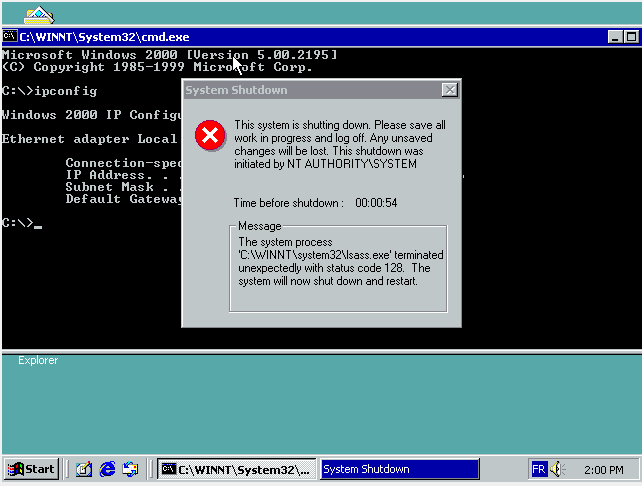
\includegraphics[scale=0.4]{Image9}
\end{figure}
Cette fois-ci, l’exploitation a réussi. Sur la machine Windows 2000, un message nous indique que le système va s'éteindre à la suite d’un arrêt “inexpliqué” du processus lsass.exe.

\subsection{Armitage}
Armitage est une interface graphique basée sur Java pour le framework Metasploit. Son objectif est d'aider les professionnels de la sécurité à mieux comprendre le piratage et à réaliser la puissance et le potentiel de Metasploit. De plus amples informations sur cet excellent projet, ainsi que son manuel complet, peuvent être obtenus sur le site officiel d'Armitage.
\begin{figure}[H]
\centering
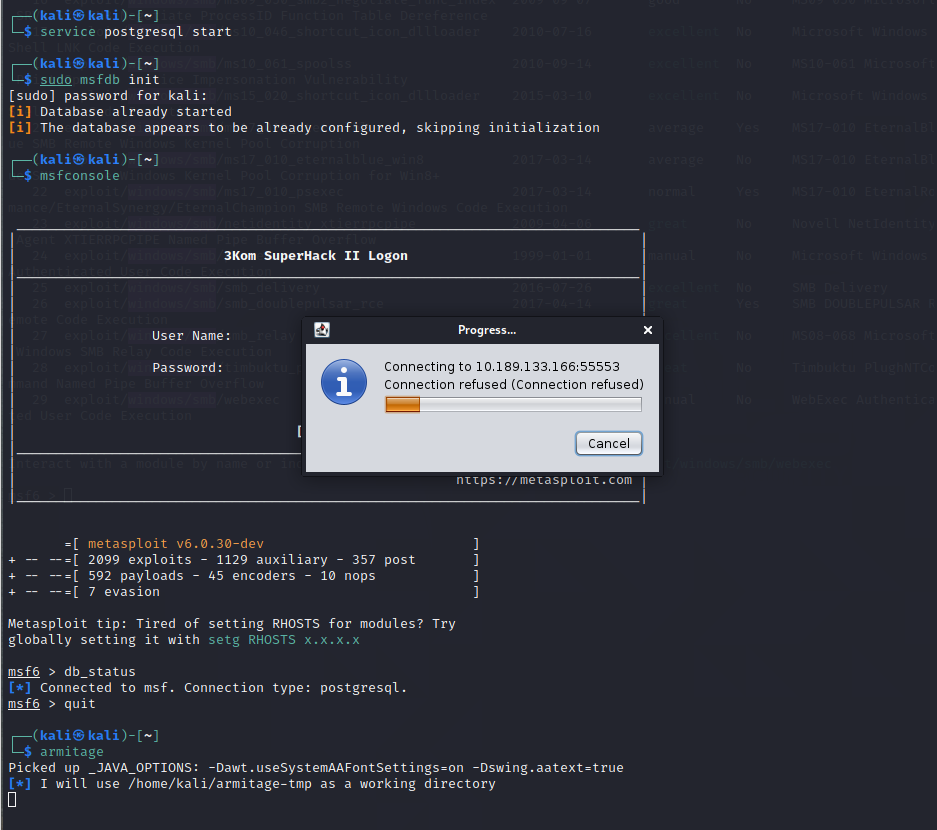
\includegraphics[scale=0.4]{Image10}
\end{figure}
La méthode de reconnaissance et d’exploitation via Armitage n’a pas pu être utilisée. Une fois les tentatives de connexions acheminées (cf la capture d’écran), la commande est restée en suspens et l’interface Armitage ne s’est pas lancée.



\end{document}